PIR-sensoren er en færdigbygget komponent, der er lavet modultest på PIR-sensoren ved at måle med et oscilloskop på output benet. På billedet \ref{lab:pir_sensor} ses det at PIR-sensoren sender det forventede output ud på ca. 3,3 VDC.    

\begin{figure}[htb]
\centering
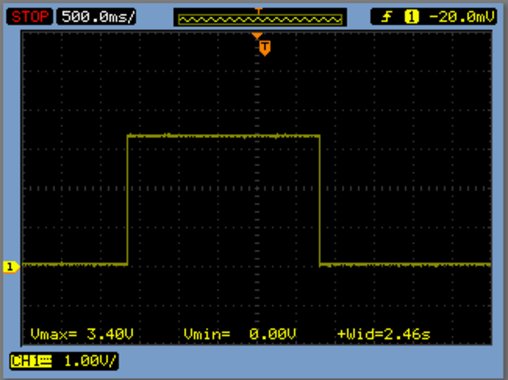
\includegraphics[width=0.60\textwidth]{filer/pics/pir_sensor}
\caption{Oscilliskop billede af PIR output-signal}
\label{lab:pir_sensor}
\end{figure}

